\chapter{Improving the Performance of Predictive Models for Compiler Heuristics}
\label{chap:clgen}


\section{Introduction}

Predictive modelling using machine learning is an effective method for building compiler heuristics, but there is a shortage of benchmarks. Typical machine learning experiments outside of the compilation field train over thousands or millions of examples. In machine learning for compilers, however, there are typically only a few dozen common benchmarks available. This limits the quality of learned models, as they have very sparse training data for what are often high-dimensional feature spaces. What is needed is a way to generate an unbounded number of training programs that finely cover the feature space. At the same time, the generated programs must be similar to the types of programs that human developers actually write, otherwise, the learning will target the wrong parts of the feature space.

This chapter introduces \emph{CLgen}, a generator for OpenCL benchmarks. Open source repositories are mined for program fragments which are used to automatically construct deep learning models for how humans write programs. The models are sampled to generate an unbounded number of runnable training programs. The quality of the programs is such that even human developers struggle to distinguish the generated programs from handwritten code. In this chapter, CLgen is used to automatically synthesise thousands of programs and show that learning over these improves the performance heterogeneous workloads using a state-of-the-art predictive model by $1.27\times$. In addition, the fine covering of the feature space automatically exposes weaknesses in the feature design which are invisible with the sparse training examples from existing benchmark suites. Correcting these weaknesses further increases workload performance by $4.30\times$.

Predictive modelling is a well-researched method for building optimisation heuristics that often exceed human experts and reduces development time~\cite{Micolet2016,Wang2014c,Magni2014,Cummins2016,Wang2009,Wen2015,Wang2010,Falch2015,Collins2012,Leather2014,Ogilvie2014a}. Figure~\ref{fig:training-a-predictive-model} shows the process by which a predictive model is constructed. A set of training programs are identified that are expected to be representative of the application domain. The programs are compiled and executed with different parameter values for the target heuristic, to determine which are the best values for each training program. Each program is also summarised by a vector of features which describe the information that is expected to be important in predicting the best heuristic parameter values. These training examples of program features and desired heuristic values are used to create a machine learning model which, when given the features from a new, unseen program, can predict good heuristic values for it.

\begin{figure}
  \centering
  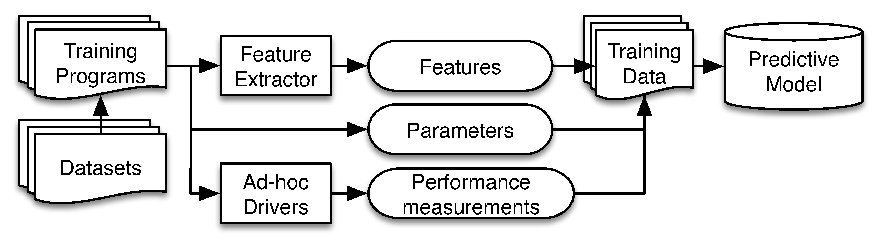
\includegraphics[width=0.9\columnwidth]{img/overview-a}%
  \caption[Training a predictive model for compiler optimisations]{%
    Training a predictive model for compiler optimisations. A model is constructed from training data, which comprises the features, performance measurements, and runtime parameters of training programs and their accompanying data sets.%
  }%
  \label{fig:training-a-predictive-model}
\end{figure}

It is common for feature vectors to contain dozens of elements. This means that a large volume of training data is needed to have adequate sampling over the feature space. Without it, the machine-learned models only capture the coarse characteristics of the heuristic, and new programs which do not lie near to training points may be wrongly predicted. The accuracy of the machine-learned heuristic is thus limited by the sparsity of available training points.

There have been efforts to solve this problem using templates. The essence of the approach is to construct a probabilistic grammar with embedded semantic actions that define a language of possible programs. New programs may be created by sampling the grammar and, through setting probabilities on the grammar productions, the sampling is biased towards producing programs from one part of the space or another. This technique is potentially completely general since a grammar might theoretically be constructed to match any desired program domain. However, despite being theoretically possible, it is not easy to construct grammars which are both suitably general and also produce programs that are in any way similar to human-written programs. It has been shown to be successful only over a highly restricted space of stencil benchmarks with little control flow or program variability~\cite{Falch2015,Cummins2016a}, or by using a very limited set of programming language features~\cite{Kosta2019}. But, it is not clear how much effort it will take, or even if it is possible for human experts to define grammars that are capable of producing human-like programs in more complex domains, without restrictions on programming language features.

The approach introduced in this chapter does not require an expert to define what human programs look like. Instead, the structure of programs is automatically inferred over a huge corpus of handwritten programs taken from open source projects. A probability distribution is constructed over sets of characters seen in human-written code. This distribution is sampled to generate new random programs which, because the distribution models human-written code, are indistinguishable from human code. These samples can be used to populate training data with an unbounded number of human-like programs, covering the space far more finely than either existing benchmark suites or even the corpus of open source projects. The approach is enabled by two recent developments:

The first is the breakthrough in effectiveness of deep learning for modelling complex structure in natural languages~\cite{Graves2013,Sutskever2014}. Deep learning is capable not just of learning the macro syntactical and semantic structure of programs, but also the nuances of how humans typically write code. It is truly remarkable when one considers that it is given no prior knowledge of the syntax or semantics of the language.

The second is the increasing popularity of public and open platforms for hosting software projects and source code. This popularity provides thousands of programming examples that are necessary to feed into the deep learning. These open source examples are not, sadly, as useful for directly learning the compiler heuristics since they are not presented in a uniform, runnable manner, nor do they typically have extractable test data. Preparing each of the thousands of open source projects to be directly applicable for learning compiler heuristics would be an insurmountable task. In addition to the program generator, CLgen, this chapter presents an accompanying host driver which generates data sets for, then executes and profiles synthesised programs.

In the course of evaluating the technique against prior work, the generator is found to be useful also for evaluating the quality of features. Since the program space is covered so much more finely than in the prior work, which only used standard benchmark suites, CLgen is able to find multiple programs with identical feature values but different best heuristic values. This indicates that the features are not sufficiently discriminative and should be extended with more information to allow those programs to be separated. Doing so significantly increases the performance of the learned heuristic.

This chapter is organised as follows: first, Section~\ref{sec:the-case-for-benchmark-generators} presents the motivation for the use of benchmark generators in predictive modelling. Then Section~\ref{sec:clgen} introduces CLgen, a generator for human-like source code. Section~\ref{sec:cldrive} describes the driver for executing synthesised source code. CLgen is evaluated first through a qualitative evaluation comparing the output to handwritten code in Section~\ref{sec:clgen-qualitative-evaluation} then quantitatively by extending the training set of a state-of-the-art machine learning optimisation heuristic. The setup of the quantitative experiments is described in Section~\ref{sec:clgen-eval-methodology} and the results in Section~\ref{sec:clgen-eval-results}. Finally, Section~\ref{sec:clgen-conclusion} concludes this chapter.


\section{The Case for Generating Benchmarks}%
\label{sec:the-case-for-benchmark-generators}

This section makes the argument for synthetic benchmarks. Frequently used benchmark suites were identified in a survey of 25 GPGPU performance tuning research papers from four top tier conferences between 2013--2016: CGO, HiPC, PACT, and PPoPP. The average number of benchmarks used in each paper is 17, and a small pool of benchmark suites account for the majority of results, illustrated in Figure~\ref{fig:benchmark-suite-distribution}. The performance of the state-of-the-art \citeauthor{Grewe2013}~\cite{Grewe2013} predictive model was evaluated across each of the 7 most frequently used benchmark suites (accounting for 94\% of results in the surveyed papers). The model predicts whether running an OpenCL kernel on the GPU provides better performance than on the CPU. The full experimental setup is described in Section~\ref{sec:clgen-eval-methodology}.

\begin{figure}
  \centering
  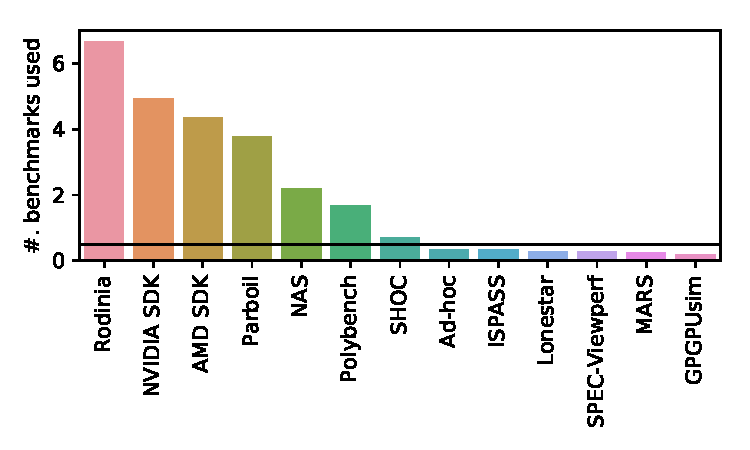
\includegraphics{img/motivation-c} %
  \caption[Benchmark counts in GPGPU research papers]{%
    The average number of benchmarks used in GPGPU research papers published between 2013-2016 in CGO, HiPC, PACT, and PPoPP conferences. The average GPGPU research paper uses 17 benchmarks, with the seven most popular benchmark suites accounting for 94\% of results.%
  }%
  \label{fig:benchmark-suite-distribution}
\end{figure}

\begin{table}
	\centering
	\rowcolors{2}{gray!25}{white}
\begin{tabular}{ | R{2.0cm} | C{1.25cm} C{1.25cm} C{1.25cm} C{1.25cm} C{1.25cm} C{1.25cm} C{1.25cm} | }
  \hline
  \rowcolor{gray!50}
  & \rotatebox[origin=c]{90}{\textbf{AMD}} & \rotatebox[origin=c]{90}{\textbf{NPB}} & \rotatebox[origin=c]{90}{\textbf{NVIDIA}} & \rotatebox[origin=c]{90}{\textbf{Parboil}} & \rotatebox[origin=c]{90}{\textbf{Polybench}} & \rotatebox[origin=c]{90}{\textbf{Rodinia}} & \rotatebox[origin=c]{90}{\textbf{SHOC}}\\
  \hline
  \textbf{AMD} & - & 38.0\% & 74.5\% & 76.7\% & 21.7\% & 45.8\% & 35.9\%\\
  \textbf{NPB} & 22.7\% & - & 45.3\% & 36.7\% & 13.4\% & 16.1\% & 23.7\%\\
  \textbf{NVIDIA} & 29.9\% & 37.9\% & - & 21.8\% & 78.3\% & 18.1\% & 63.2\%\\
  \textbf{Parboil} & 89.2\% & 28.2\% & 28.2\% & - & 41.3\% & 73.0\% & 33.8\%\\
  \textbf{Polybench} & 58.6\% & 30.8\% & 45.3\% & 11.5\% & - & 43.9\% & 12.1\%\\
  \textbf{Rodinia} & 39.8\% & 36.4\% & 29.7\% & 36.5\% & 46.1\% & - & 59.9\%\\
  \textbf{SHOC} & 42.9\% & 71.5\% & 74.1\% & 41.4\% & 35.7\% & 81.0\% & -\\
  \hline
\end{tabular}

	\caption[Cross-validation of benchmark suites on a predictive model]{%
		Performance relative to the optimal of the \citeauthor{Grewe2013} predictive model across different benchmark suites on an AMD GPU. The columns show the suite used for training; the rows show the suite used for testing. On average, a predictive model trained on one benchmark suite and tested on another achieves only 49\% of the optimal performance.%
	}
	\label{tab:cpu-gpu-benchmarks-crossvalidate}
\end{table}

Table~\ref{tab:cpu-gpu-benchmarks-crossvalidate} summarises the results. The performance of a model trained on one benchmark suite and used to predict the mapping for another suite is generally poor. The benchmark suite which provides the best results, NVIDIA SDK, achieves on average only 49\% of the optimal performance. The worst case is when training with Parboil to predict the optimal mappings for Polybench, where the model achieves only 11.5\% of the optimal performance. From this, it is clear that models trained on one benchmark suite fail to generalise across other suites.

This problem is caused both by the limited number of benchmarks contained in each suite, and the distribution of benchmarks within the feature space. Figure~\ref{fig:pca-benchmarks} shows the feature space of the Parboil benchmark suite, showing whether, for each benchmark, the model was able to correctly predict the appropriate optimisation. Principal Component Analysis is used to reduce the multi-dimensional feature space to aid visualisation.

\begin{figure}
  \centering
  % The empty square brackets are required to keep the (a) and (b) subfloat labels.
  \subfloat[][]{%
    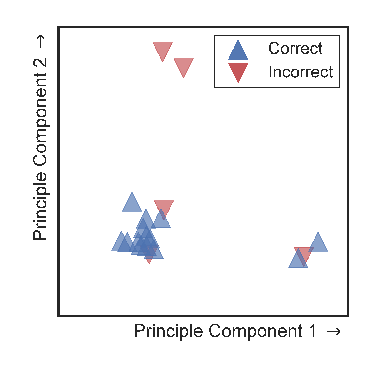
\includegraphics[width=.55\columnwidth]{img/motivation-a}%
    \label{fig:pca-benchmarks-a}%
  }%
  \\*
  \subfloat[][]{%
    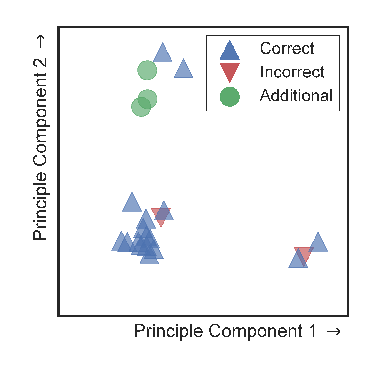
\includegraphics[width=.55\columnwidth]{img/motivation-b}%
    \label{fig:pca-benchmarks-b}%
  }%
  \caption[Identifying and correcting outliers in a benchmark suite]{%
    A two dimensional projection of the \citeauthor{Grewe2013} feature space, showing predictive model results over Parboil benchmarks on an NVIDIA GPU. Two outliers in~\protect\subref{fig:pca-benchmarks-a} are incorrectly predicted due to the lack of nearby observations. The addition of neighbouring observations in~\protect\subref{fig:pca-benchmarks-b} corrects this.%
  }%
  \label{fig:pca-benchmarks}
\end{figure}

As seen in Figure~\ref{fig:pca-benchmarks-a}, there is a dense cluster of neighbouring benchmarks, a smaller cluster of three benchmarks, and two outliers. The lack of neighbouring observations means that the model is unable to learn a good heuristic for the two outliers, which leads to them being incorrectly optimised. In Figure~\ref{fig:pca-benchmarks-b}, additional benchmarks which are neighbouring in the feature space were hand-selected and the model retrained. The addition of these observations (and the information they provide about that part of the feature space) causes the two outliers to be correctly optimised. Such outliers can be found in all of the benchmark suites of Table~\ref{tab:cpu-gpu-benchmarks-crossvalidate}.

These results highlight the significant effect that the number and distribution of training programs have on the quality of predictive models. Without good coverage of the feature space, any machine learning methodology is unlikely to produce high-quality heuristics, suitable for general use on arbitrary real applications, or even applications from different benchmark suites. The novel approach described in the next section addresses this problem by generating an unbounded number of programs to cover the feature space with fine granularity.


\section[CLgen: A System for Generating OpenCL Benchmarks]{CLgen: A System for Generating OpenCL\\*Benchmarks}
\label{sec:clgen}

This section introduces CLgen, an undirected, general-purpose program synthesizer. It adopts and augments recent advanced techniques from deep learning to learn over massive code-bases. In contrast to existing grammar- and template-based approaches, CLgen is entirely probabilistic. The system \emph{learns} to program using recurrent neural networks which model the semantics and usage of a huge corpus of code fragments in the target programming language.


\subsection{Overview}

Figure~\ref{fig:clgen-pipeline} provides an overview of the program synthesis and execution pipeline. CLgen learns the semantics and structure from over a million lines of handwritten code from GitHub, and synthesises programs through a process of iterative model sampling. A host driver, described in Section~\ref{sec:cldrive}, executes the synthesised programs to gather performance data for use in predictive modelling. While the approach is demonstrated using OpenCL, it is language-agnostic. This approach extends the state-of-the-art by providing a general-purpose solution for benchmark synthesis, leading to better and more accurate predictive models.

Section~\ref{subsec:opencl-lang-corpus} describes the assembly of a language corpus, Section~\ref{sec:learning-opencl} describes the application of deep learning over this corpus, and Section~\ref{subsec:synthesizing-opencl} describes the process of synthesising programs.

\begin{figure}
  \centering%
  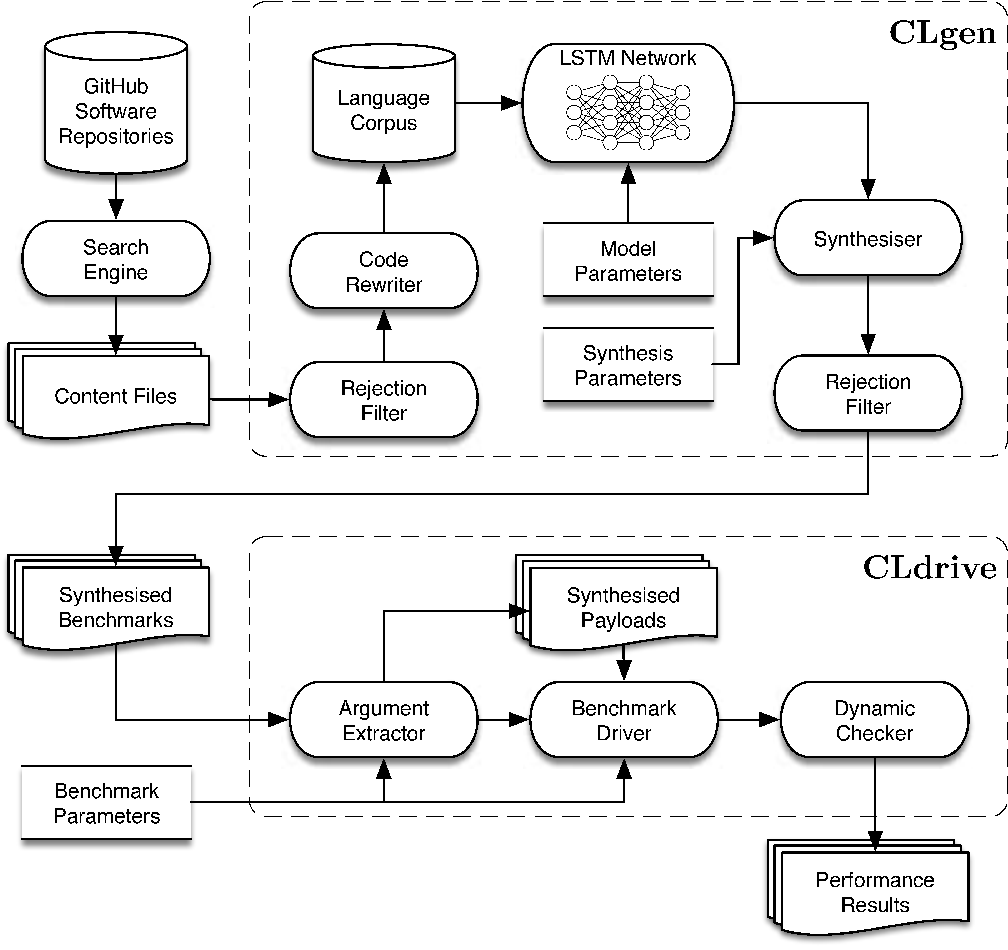
\includegraphics[width=\columnwidth]{img/clgen-pipeline}%
  \caption[Benchmark synthesis and execution pipeline]{%
    The benchmark synthesis and execution pipeline. Software is mined from GitHub; this is used to construct a language model from which new programs may be synthesised; a benchmark driver is used to produce performance results.%
  }%
  \label{fig:clgen-pipeline}
\end{figure}


\subsection{An OpenCL Language Corpus}
\label{subsec:opencl-lang-corpus}

Deep learning requires large data sets~\cite{LeCun2015}. For the purpose of modelling a programming language, this means assembling a large collection of real, handwritten source codes. OpenCL codes are assembled by mining public repositories on the popular code hosting site GitHub.

This is itself a challenging task since OpenCL is an embedded language, meaning device code is often difficult to untangle since GitHub does not presently recognise it as a searchable programming language. A search engine was developed which attempts to identify and download standalone OpenCL files through a process of file scraping and recursive header inlining. The result is a 2.8 million line data set of 8078 ``content files'' which potentially contain OpenCL code, originating from 793 GitHub repositories.

The raw data set extracted from GitHub is then pruned using a custom toolchain developed for rejection filtering and code rewriting, built on LLVM.


\paragraph*{Rejection Filter}
\label{subsubsec:opencl-rejection-filter}

The rejection filter accepts as input a content file and returns whether or not it contains compilable, executable OpenCL code. To achieve this, it attempts to compile the input to NVIDIA PTX byte code and performs static analysis to ensure a minimum static instruction count of three. Any inputs which do not compile or contain fewer than three instructions are discarded.

During initial development, it became apparent that isolating the OpenCL device code leads to a higher-than-expected discard rate (that is, seemingly valid OpenCL files being rejected). Through analysing 148k lines of compilation errors, a large number of failures were discovered to be caused by undeclared identifiers, a result of isolating device code. 50\% of undeclared identifier errors in the GitHub dataset were caused by only 60 unique identifiers. To address this, a \emph{shim header} was developed which contains inferred values for common type definitions (e.g. \texttt{FLOAT\_T}), and common constants (e.g. \texttt{WGSIZE}), shown in Listing~\ref{lst:opencl-shim-header}.

\begin{listing}
\inputminted{c}{lst/opencl-shim-header.h}
\caption[The \emph{shim} header file for compiling OpenCL from GitHub]{An overview of the \emph{shim} header file, providing commonly used type aliases and constants for compiling OpenCL files taken on GitHub.}
\label{lst:opencl-shim-header}
\end{listing}

Injecting the shim decreases the discard rate from 40\% to 32\%, responsible for an additional 88k lines of code in the final language corpus. The resulting data set is 2.0 million lines of compilable OpenCL source code.


\paragraph*{Code Rewriter}
\label{subsubsec:clgen-rewriter}

Programming languages have few of the issues of semantic interpretation present in natural language, though there remain many sources of variance at the syntactic level. For example, the presence and content of comments in code, and the choice of identifying names given to variables. For the purposes of generative modelling, these ambiguities are considered to be \emph{non-functional variance}. The \emph{code rewriter} is a tool developed to normalise code of these variances so as to make code more amenable to machine learning. This is a three-step process:

\begin{enumerate}
  \item The source file is pre-processed using the compiler front-end to remove macros, conditional compilation, and source comments.
  \item Identifiers are rewritten to have a short but unique name based on their order of appearance, using the sequential series $\{a,\allowbreak b,\allowbreak c,\allowbreak \ldots,\allowbreak aa,\allowbreak ab,\allowbreak ac,\allowbreak \ldots\}$ for variables and $\{A,\allowbreak B,\allowbreak C,\allowbreak \ldots,\allowbreak AA,\allowbreak AB,\allowbreak AC,\allowbreak \ldots\}$ for functions. This process isolates the syntactic structure of the code, and unlike prior work~\cite{Allamanis2013a}, this rewrite method preserves program behaviour. Language built-ins (e.g. \texttt{get\_global\_id}, \texttt{asin}) are not rewritten.
  \item A variant of the Google C++ code style~\cite{Weinberger2011} is enforced to ensure consistent use of braces, parentheses, and white space.
\end{enumerate}

An example of the code rewriting process is shown in Listings~\ref{lst:code-rewriting-before} and~\ref{lst:code-rewriting-after}. A side effect of this process is a reduction in code size, largely due to the removal of comments and excess white space. The final language corpus contains 1.3 million lines of transformed OpenCL, consisting of 9487 kernel functions. Identifier renaming reduces the \emph{bag-of-words} vocabulary size --- the number of unique entries in the tokenised corpus --- by 84\%.

\begin{listing}
  \inputminted{opencl_lexer.py:OpenCLLexer -x}{lst/clgen-rewrite-before.cl}
  \caption[Example OpenCL content file from GitHub]{An example OpenCL content file prior to code rewriting.}
  \label{lst:code-rewriting-before}
\end{listing}

\begin{listing}
  \inputminted{opencl_lexer.py:OpenCLLexer -x}{lst/clgen-rewrite-after.cl}
  \caption[OpenCL content file after rewriting]{The example OpenCL content file of Listing~\ref{lst:code-rewriting-before} after code rewriting. Conditional compilation has been removed, the variables and functions renamed, and a code style enforced.}
  \label{lst:code-rewriting-after}
\end{listing}


\subsection{Learning OpenCL}
\label{sec:learning-opencl}

Generating valid, executable program code is an ambitious and challenging goal for unsupervised machine learning. CLgen employs state-of-the-art deep language modelling techniques to achieve this task.

The Long Short-Term Memory (LSTM)~\cite{Hochreiter1997} architecture of Recurrent Neural Network~\cite{Sundermeyer2012,Mikolov2015} is used to learn a character-level language model over the corpus of OpenCL compute kernels. The LSTM network architecture comprises recurrent layers of \emph{memory cells}, each consisting of input, output, and forget gates, and an output layer providing normalised probability values from a 1-of-K coded vocabulary~\cite{Graves2005}.

A 3-layer LSTM network is used with 2048 nodes per layer, implemented in Torch. This 17-million parameter model is trained using \textit{Stochastic Gradient Descent} for 50 epochs, using an initial learning rate of 0.002, decaying by a factor of one half every 5 epochs. Training took three weeks on a single machine using an NVIDIA GTX Titan, with a final model size of 648MB\footnote{No effort was made to minimise training time. Subsequent work using tuned parameters and a more efficient model implementation in TensorFlow has reduced this time considerably.}. Training the network is a one-off cost, and is parallelisable across devices. The trained network can be deployed to lower-compute machines for use.


\subsection{Synthesising Source Code}
\label{subsec:synthesizing-opencl}

\begin{algorithm}
  \begin{algorithmic}[1]
\Require LSTM model $M$, maximum kernel length $n$.
\Ensure Completed sample string $S$.
\State $S \gets$``\texttt{\_\_kernel void A(const int a) \{}''\algorithmiccomment{Seed text from argument specification}
\State $d \gets 1$\algorithmiccomment{Initial code block depth}
\For{$i \gets |S|$ \textbf{to} $n$}
  \State $c \gets PredictCharacter(M, S)$\algorithmiccomment{Generate new character}
  \If{$c = $``\texttt{\{}''}
    \State $d \gets d+1$\algorithmiccomment{Entered code block, increase depth}
  \ElsIf{$c = $``\texttt{\}}''}
    \State $d \gets d-1$\algorithmiccomment{Exited code block, decrease depth}
  \EndIf
  \State $S \gets S + c$\algorithmiccomment{Append new character to sample}
  \If{$depth = 0$}
    \State \textbf{break}\algorithmiccomment{Exited function block, stop sampling}
  \EndIf

\EndFor
\end{algorithmic}

  \caption[Sampling a candidate kernel from a seed text]{Using an LSTM model to sample a candidate OpenCL kernel.}
  \label{alg:clgen-synthesis}
\end{algorithm}

OpenCL compute kernels are synthesised by iteratively sampling the learned language model. Two modes for model sampling are supported: the first involves providing an \emph{argument specification}, stating the data types and modifiers of all kernel arguments. When an argument specification is provided, the model synthesises kernels matching this signature. In the second sampling mode, this argument specification is omitted, allowing the model to synthesise compute kernels of arbitrary signatures, dictated by the distribution of argument types within the language corpus.

\begin{listing}
  \inputminted{opencl_lexer.py:OpenCLLexer -x}{lst/clgen-sample-a.cl}
  \caption[Synthesised vector operation with branching and synchronisation]{CLgen-synthesised vector operation with branching and synchronisation.}
  \label{lst:clgen-sample-a}
\end{listing}

\begin{listing}
  \inputminted{opencl_lexer.py:OpenCLLexer -x}{lst/clgen-sample-b.cl}
  \caption[Synthesised zip operation]{CLgen-synthesised zip operation which computes $c_i = 3a_i + 2b_i + 4$.}
  \label{lst:clgen-sample-b}
\end{listing}

\begin{listing}
  \inputminted{opencl_lexer.py:OpenCLLexer -x}{lst/clgen-sample-c.cl}
  \caption[Synthesised partial reduction operation]{CLgen-synthesised partial reduction over reinterpreted vector type.}
  \label{lst:clgen-sample-c}
\end{listing}

In either mode, a \emph{seed} text is generated and the model sampled, character by character, until the end of the compute kernel is reached, or until a predetermined maximum number of characters is reached. Algorithm~\ref{alg:clgen-synthesis} illustrates this process. The same rejection filter as is used during corpus assembly that either accepts or rejects the sample as a candidate synthetic benchmark. Listings~\ref{lst:clgen-sample-a},~\ref{lst:clgen-sample-b}, and~\ref{lst:clgen-sample-c} show three examples of unique compute kernels generated in this manner from an argument specification of three single-precision floating-point arrays and a read-only signed integer. The quality of synthesised code is evaluated in Section~\ref{sec:clgen-qualitative-evaluation}.


\section{CLdrive: A System for Driving Arbitrary OpenCL Kernels}
\label{sec:cldrive}

This section presents \emph{CLdrive}, a host driver developed to gather performance data from synthesised CLgen code. The driver accepts as input an OpenCL kernel, generates \emph{payloads} of user-configurable sizes, then executes the kernel using the generated payloads so as to collect kernel runtimes, and to provide dynamic checking of kernel behaviour.


\subsection{Generating Data Payloads}

A \emph{payload} encapsulates all of the arguments of an OpenCL compute kernel. After parsing the input kernel to derive argument types, a rule-based approach is used to generate synthetic payloads. For a given global size $S_g$: host buffers of $S_g$ elements are allocated and populated with random values for global pointer arguments, device-only buffers of $S_g$ elements are allocated for local pointer arguments, integral arguments are given the value $S_g$, and all other scalar arguments are given random values. Host to device data transfers are enqueued for all non-write-only global buffers, and all non-read-only global buffers are transferred back to the host after kernel execution.


\subsection{Dynamic Checker}

A class of programs are defined as performing \emph{useful work} if they predictably compute some result. For the purpose of performance benchmarking the values computed by a program are of little interest, so a low-overhead runtime behaviour check is used to validate that a synthesised program does useful work based on the outcome of four executions of a tested program:

\begin{enumerate}
\item Create 4 equal size payloads $A_{1in}$, $B_{1in}$, $A_{2in}$,
  $B_{2in}$, subject to restrictions: $A_{1in}=A_{2in}$,
  $B_{1in}=B_{2in}$, $A_{1in} \ne B_{1in}$.
\item Execute kernel $k$ 4 times: $k(A_{1in}) \rightarrow A_{1out}$,
  $k(B_{1in}) \rightarrow B_{1out}$,
  $k(A_{2in}) \rightarrow A_{2out}$,
  $k(B_{2in}) \rightarrow B_{2out}$.
\item Assert that:
  \begin{itemize}
  \item $A_{1out} \ne A_{1in}$ and $B_{1out} \ne B_{1in}$, else $k$ has no
  output (for these inputs).%
  \item $A_{1out} \ne B_{1out}$ and $A_{2out} \ne B_{2out}$, else $k$ is input insensitive t (for these inputs).%
  \item $A_{1out}=A_{2out}$ and $B_{1out}=B_{2out}$, else $k$ is
  non-deterministic.
  \end{itemize}
\end{enumerate}

Equality checks for floating point values are performed with an appropriate epsilon to accommodate rounding errors, and a timeout threshold is also used to catch kernels which are non-terminating. The method is based on random differential testing~\cite{McKeeman1998}, though I emphasise that this is not a general purpose approach and is tailored specifically for benchmarking for performance characterisation. For example, one would anticipate a false positive rate for kernels with subtle sources of non-determinism which more thorough methods may expose~\cite{Betts2012,Price2015,Sorensen2016}, however for the purpose of performance modelling, such methods were deemed unnecessary.


\section{Qualitative Evaluation of Generated Programs}
\label{sec:clgen-qualitative-evaluation}

This section evaluates the quality of programs synthesised by CLgen by their likeness to handwritten code.


\subsection{Methodology}

Judging whether a piece of code has been written by a human is a challenging task for a machine, so a methodology was adopted from artificial intelligence research based on the \emph{Turing Test}~\cite{Gao2015a,Zhang2016,Vinyals}. If the output of CLgen is human-like code, it reasons that a human judge will be unable to distinguish it from handwritten code.

A double-blind test was devised in which 15 volunteer OpenCL developers from industry and academia were shown 10 OpenCL kernels each. Participants were tasked with judging whether, for each kernel, they believed it to have been written by hand or by machine. Kernels were randomly selected for each participant from two equal sized pools of synthetically generated and handwritten code from GitHub. The samples from GitHub were vetted to ensure that they were indeed handwritten and not generated by machine or template (such vetting is a manual process and was not applied during the assembly of the model training corpus). The code rewriting process was applied to all kernels to remove comments and ensure uniform identifier naming. The participants were divided into two groups of 10 and 5 members, with the larger group reviewing synthetic code generated CLgen. The smaller group acted as a control group, reviewing synthetic code generated by CLSmith~\cite{Lidbury2015a}, an OpenCL program generator for differential testing\footnote{An online version of this test is available at \emph{https://chriscummins.cc.uk/s/human\_or\_robot/}.}.


\subsection{Experimental Results}

Each participant's answers were scored. The average score of the control group is 96\% (stdev.\ 9\%), an unsurprising outcome as programs generated using CLSmith for testing have multiple ``tells''; for example, they make much heavier use of \texttt{struct}s than is typical, they use unusual combinations of programming language features, and their only input is a single \texttt{ulong} pointer. There were no false positives (synthetic code labelled human) for CLSmith, only false negatives (human code labelled synthetic).

With CLgen synthesised programs, the average score was 52\% (stdev.\ 17\%), and the ratio of errors was even. This suggests that CLgen code is indistinguishable from handwritten programs, with human judges scoring no better than random chance.


\section{Experimental Methodology}
\label{sec:clgen-eval-methodology}

The synthetic benchmark generator described in this chapter aims to improve the performance predictive models by augmenting their training data so as to provide a finer grained exploration of the feature space then would otherwise be possible. To test the hypothesis that CLgen-generated benchmarks are \emph{useful for training}, an experiment was designed in which a state-of-the-art predictive model was trained and evaluated with and without the addition of synthetic benchmarks and the performance compared.


\subsection{Experimental Setup}


\paragraph*{Predictive Model}

To evaluate the efficacy of synthetic benchmarks for training, the predictive model of \citeauthor{Grewe2013} is used~\cite{Grewe2013}. The predictive model is used to determine the optimal mapping of a given OpenCL kernel to either a GPU or CPU. It uses supervised learning to construct a decision tree with a combination of static and dynamic kernel features extracted from source code and the OpenCL runtime, detailed in Table~\ref{tab:clgen-cgo13-features}.

\begin{table}
  \centering%
  \subfloat[Individual code features]{%
  \rowcolors{2}{gray!25}{white}
  \begin{tabular}{| l c l |}
    \hline
    \rowcolor{gray!50}
    \textbf{Name} & \textbf{Type} & \textbf{Description} \\
    \hline
    \texttt{comp} & static & \#. compute operations \\
    \texttt{mem} & static & \#. accesses to global memory \\
    \texttt{localmem} & static & \#. accesses to local memory \\
    \texttt{coalesced} & static & \#. coalesced memory accesses \\
    \texttt{transfer} & dynamic & size of data transfers \\
    \texttt{wgsize} & dynamic & \#. work-items per kernel \\
    \hline
  \end{tabular}%
  \label{tab:clgen-cgo13-features-raw}%
}\\*
\subfloat[Combinations of raw features]{%
  \rowcolors{2}{gray!25}{white}
  \begin{tabular}{| l l l |}
    \hline
    \rowcolor{gray!50}
    \textbf{Name} & \textbf{Formulation} & \textbf{Description} \\
    \hline
    \texttt{F1} & \texttt{transfer/(comp+mem)} & Communication-computation ratio \\
    \texttt{F2} & \texttt{coalesced/mem} & \% Coalesced memory accesses \\
    \texttt{F3} & \texttt{(localmem/mem)$\times$wgsize} & Memory access ratio $\times$ \#.\ work-items \\
    \texttt{F4} & \texttt{comp/mem} & Computation-memory ratio\\
    \hline
  \end{tabular}%
  \label{tab:clgen-cgo13-features-combined}%
}
%
  \caption[\citeauthor{Grewe2013} features for heterogeneous device mapping]{%
    Features used by \citeauthor{Grewe2013} to predict CPU/GPU mapping of OpenCL kernels. The features are extracted using a custom analysis pass built using LLVM.
  }%
  \label{tab:clgen-cgo13-features} %
\end{table}


\paragraph*{Benchmarks}

As in~\cite{Grewe2013}, the model is tested on the NAS Parallel Benchmarks (NPB)~\cite{Bailey1991a}. The hand-optimised OpenCL implementation of \citeauthor{Seo2011} \cite{Seo2011} is used. In~\cite{Grewe2013} the authors augment the training set of the predictive model with 47 additional kernels taken from 4 GPGPU benchmark suites. To more fully sample the program space, a much larger collection of 142 kernels is used, summarised in Table~\ref{tab:cgo17-benchmarks}. These additional programs are taken from all 7 of the most frequently used benchmark suites identified in Section~\ref{sec:the-case-for-benchmark-generators}. None of these programs were used to train CLgen. This brings the total number of OpenCL benchmark kernels used in the evaluation to 256. 1,000 kernels were synthesised with CLgen to use as additional benchmarks.

\begin{table}
  \centering%
  \rowcolors{2}{gray!25}{white}
\begin{tabular}{| l r r r |}
  \hline
  \rowcolor{gray!50}
  & \textbf{Version} & \textbf{\#. benchmarks} & \textbf{\#. kernels}\\
  \hline
  \textbf{NPB (SNU~\cite{Seo2011})} & 1.0.3 & 7 & 114 \\
  \textbf{Rodinia~\cite{Che2009}} & 3.1 & 14 & 31 \\
  \textbf{NVIDIA SDK} & 4.2 & 6 & 12 \\
  \textbf{AMD SDK} & 3.0 & 12 & 16 \\
  \textbf{Parboil~\cite{Stratton2012}} & 0.2 & 6 & 8 \\
  \textbf{PolyBench~\cite{Grauer-Gray2012}} & 1.0 & 14 & 27 \\
  \textbf{SHOC~\cite{Danalis2010}} & 1.1.5 & 12 & 48 \\
  \textbf{Total} & - & 71 & 256 \\
  \hline
\end{tabular}

  \caption[Benchmarks used in evaluation]{List of benchmarks used to train and evaluate the \citeauthor{Grewe2013} predictive model.} %
  \label{tab:cgo17-benchmarks} %
\end{table}


\paragraph*{Experimental Platforms}

Two 64-bit CPU-GPU systems are used to evaluate the approach, detailed in Table~\ref{tab:cgo17-platforms}. One system has an AMD GPU and uses OpenSUSE 12.3; the other is equipped with an NVIDIA GPU and uses Ubuntu 16.04. Both platforms were unloaded.

\begin{table}
  \centering %
  \rowcolors{2}{gray!25}{white}
\begin{tabular}{| l l l l |}
  \hline
  \rowcolor{gray!50}
  & \textbf{Intel CPU} & \textbf{AMD GPU} & \textbf{NVIDIA GPU} \\
  \hline
  \textbf{Model} & Core i7-3820 & Tahiti 7970 & GTX 970 \\
  \textbf{Frequency} & 3.6 GHz & 1000 MHz & 1050 MHz \\
  \textbf{\#. Cores} & 4 & 2048 & 1664 \\
  \textbf{Memory} & 8 GB & 3 GB & 4 GB \\
  \textbf{Throughput} & 105 GFLOPS & 3.79 TFLOPS & 3.90 TFLOPS \\
  \textbf{Driver} & AMD 1526.3 & AMD 1526.3 & NVIDIA 361.42 \\
  \textbf{Compiler} & GCC 4.7.2 & GCC 4.7.2 & GCC 5.4.0 \\
  \hline
\end{tabular}

  \caption[Experimental platforms used in evaluation]{Experimental platforms used to evaluate the \citeauthor{Grewe2013} predictive model.}
  \label{tab:cgo17-platforms}
\end{table}


\paragraph*{Data sets}

The NPB and Parboil benchmark suites are packaged with multiple data sets. All of the packaged data sets are used (5 per program in NPB, 1-4 per program in Parboil). For all other benchmarks, the default data sets are used. The CLgen host driver was configured to synthesise payloads between 128B-130MB, approximating that of the dataset sizes found in the benchmark programs.


\subsection{Methodology}

The same methodology is used as in~\cite{Grewe2013}. Each experiment is repeated five times and the average execution time is recorded. The execution time includes both device compute time and the data transfer overheads.

Models are evaluated using \emph{leave-one-out cross-validation}. For each benchmark, a model is trained on data from all other benchmarks and used to predict the mapping for each kernel and dataset in the excluded program. The process is repeated with and without the addition of synthetic benchmarks in the training data. Only the real handwritten benchmarks are used to test model predictions, the synthetic benchmarks are not used.


\section{Experimental Results}
\label{sec:clgen-eval-results}

The effectiveness of synthetic benchmarks is evaluated on two heterogeneous systems. First, the performance of a state-of-the-art predictive model~\cite{Grewe2013} is compared with and without the addition of synthetic benchmarks, then synthetic benchmarks are shown to expose weaknesses in the feature design and how these can be addressed to develop a better model. Finally, the ability of CLgen to explore the program feature space is compared against a state-of-the-art program generator.


\subsection{Performance Evaluation}

\begin{figure}
  \centering %
  \subfloat[][AMD Tahiti 7970]{%
    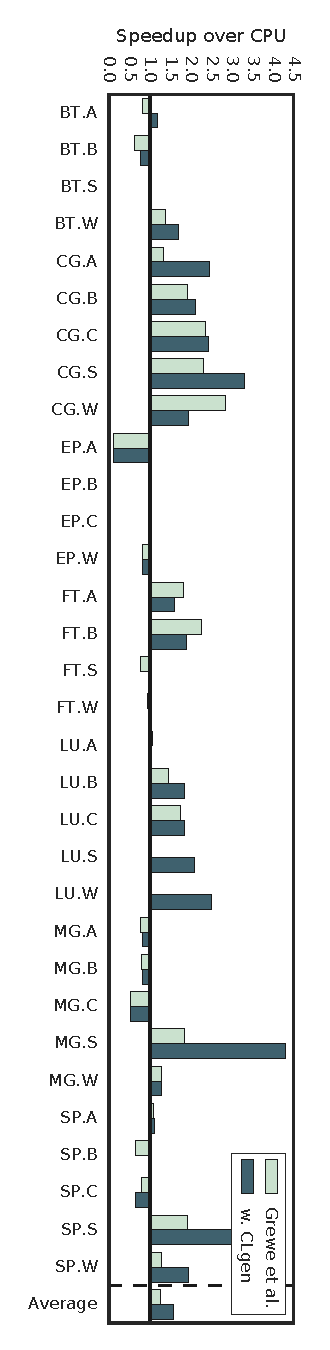
\includegraphics[width=.32\textwidth,angle=0]{img/ex1-A}%
    \label{fig:npb-amd}}%
  \subfloat[][NVIDIA GTX 970]{%
    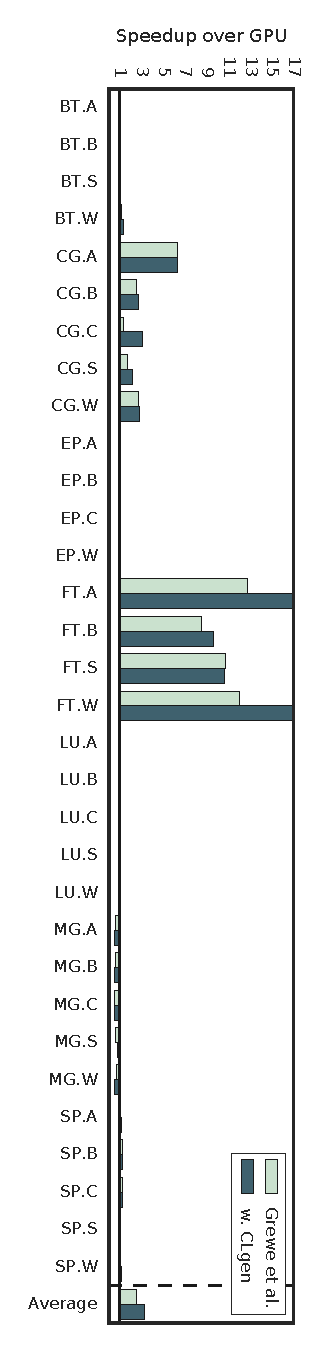
\includegraphics[width=.32\textwidth,angle=0]{img/ex1-B}%
    \label{fig:npb-nvidia}}%
  \caption[Speedup of predictions with and without synthetic benchmarks]{%
    Speedup of programs using \citeauthor{Grewe2013} predictive model with and without synthetic benchmarks. The predictive model outperforms the best static device mapping by a factor of $1.26\times$ on AMD and $2.50\times$ on NVIDIA. The addition of synthetic benchmarks improves the performance to $1.57\times$ on AMD and $3.26\times$ on NVIDIA.%
  }%
  \label{fig:npb} %
\end{figure}

Figure~\ref{fig:npb} shows speedups of the \citeauthor{Grewe2013} predictive model over the NAS Parallel Benchmark suite with and without the addition of synthesised benchmarks for training. Speedups are calculated relative to the best single-device mapping for each experimental platform, which is CPU-only for AMD and GPU-only for NVIDIA. The fine-grained coverage of the feature space which synthetic benchmarks provide improves performance dramatically for the NAS benchmarks. Across both systems, an average speedup of $2.42\times$ is achieved with the addition of synthetic benchmarks, with prediction improvements over the baseline for 62.5\% of benchmarks on AMD and 53.1\% on NVIDIA.

The strongest performance improvements are on NVIDIA with the \texttt{FT} benchmark which suffers greatly under a single-device mapping. However, the performance on AMD for the same benchmark slightly degrades after adding the synthetic benchmarks. This issue is addressed in the next section.


\subsection{Extending the Predictive Model}
\label{subsec:eval-extended}

Feature designers are bound to select as features only properties which are significant for the handful of benchmarks they test on, which limits a model's ability to generalise over a wider range of programs. This is found to be the case with the \citeauthor{Grewe2013} model. The addition of automatically generated programs exposed two distinct cases where the model failed to generalise as a result of overspecialising to the NPB suite.

The first case is that the feature \texttt{F3} of Table~\ref{tab:clgen-cgo13-features} is sparse on many programs. This is a result of the NPB implementation's heavy exploitation of local memory buffers and the method by which they combined features (speculatively, this may have been a necessary dimensionality reduction in the presence of sparse training programs). A simple countermeasure is taken to address this by extending the model to use the raw feature values in addition to the combined features.

The second case is that some CLgen-generated programs had identical feature values as in the benchmark set, but had different \emph{behaviour} (i.e. optimal mappings). Listing~\ref{lst:zero-b} shows one example of a CLgen benchmark which is indistinguishable in the feature space to one of the of existing benchmarks --- AMD's Fast Walsh-Hadamard transform, Listing~\ref{lst:amd-fast-walsh-transform} --- but with different behaviour. Comparing the program fragments reveals two primary differences: Listing~\ref{lst:amd-fast-walsh-transform} contains indirect memory accesses that cannot be coalesced, and Listing~\ref{lst:zero-b} contains a branching operation whereas Listing~\ref{lst:amd-fast-walsh-transform} has linear control flow. Neither of these properties are captured by the features used in the \citeauthor{Grewe2013} model. In the case of the branching operation, we can speculate that the choice not to consider control flow was an intentional decision by the authors given that the NPB programs on which the model was initially evaluated on are implemented in a manner which aggressively minimises branching. However, as demonstrated through CLgen's automatic exploration of the program space, such a decision hinders the model's ability to generalize to a range of programs. To counter this the predictive model was extended with an additional feature containing a static count of branching operations in a kernel.

\begin{listing}
  \inputminted{opencl_lexer.py:OpenCLLexer -x}{lst/amd-fast-walsh-transform.cl}
  \caption[AMD's Fast Walsh Transform kernel]{AMD's Fast Walsh Transform benchmark kernel. In the \citeauthor{Grewe2013} feature space this is indistinguishable from the CLgen program of Listing~\ref{lst:zero-b}, but has very different runtime behaviour and optimal device mapping. The addition of a branching feature fixes this.}
  \label{lst:amd-fast-walsh-transform}
\end{listing}

\begin{listing}
  \inputminted{opencl_lexer.py:OpenCLLexer -x}{lst/amd-fast-walsh-transform-equivalent.cl}
  \caption[Synthesised program with same features as an AMD benchmark]{In the \citeauthor{Grewe2013} feature space, this CLgen program is indistinguishable from the AMD Fast Walsh–Hadamard transform benchmark kernel of Listing~\ref{lst:amd-fast-walsh-transform}, but has very different runtime behaviour and optimal device mapping. The addition of a branching feature fixes this.}
  \label{lst:zero-b}
\end{listing}

\newpage
Figure~\ref{fig:ex2} shows speedups of the model with the extended feature set across all seven of the benchmark suites used in Section~\ref{sec:the-case-for-benchmark-generators}. Model performance, even on this tenfold increase of benchmarks, is good. There are three benchmarks on which the model performs poorly: \texttt{MatrixMul}, \texttt{cutcp}, and \texttt{pathfinder}. Each of those programs makes heavy use of loops, which changes the dynamic behaviour of the programs in ways that the static code features of the model are unlikely to capture. This could be addressed by extracting dynamic instruction counts using profiling, but this is beyond the scope of this work. It is not the aim of this work to perfect the predictive model but to show the performance improvements associated with training on synthetic programs. To this extent, the proposed approach is successful, achieving average speedups of $3.56\times$ on AMD and $5.04\times$ on NVIDIA across a very large test set.

\begin{figure}
  \centering%
  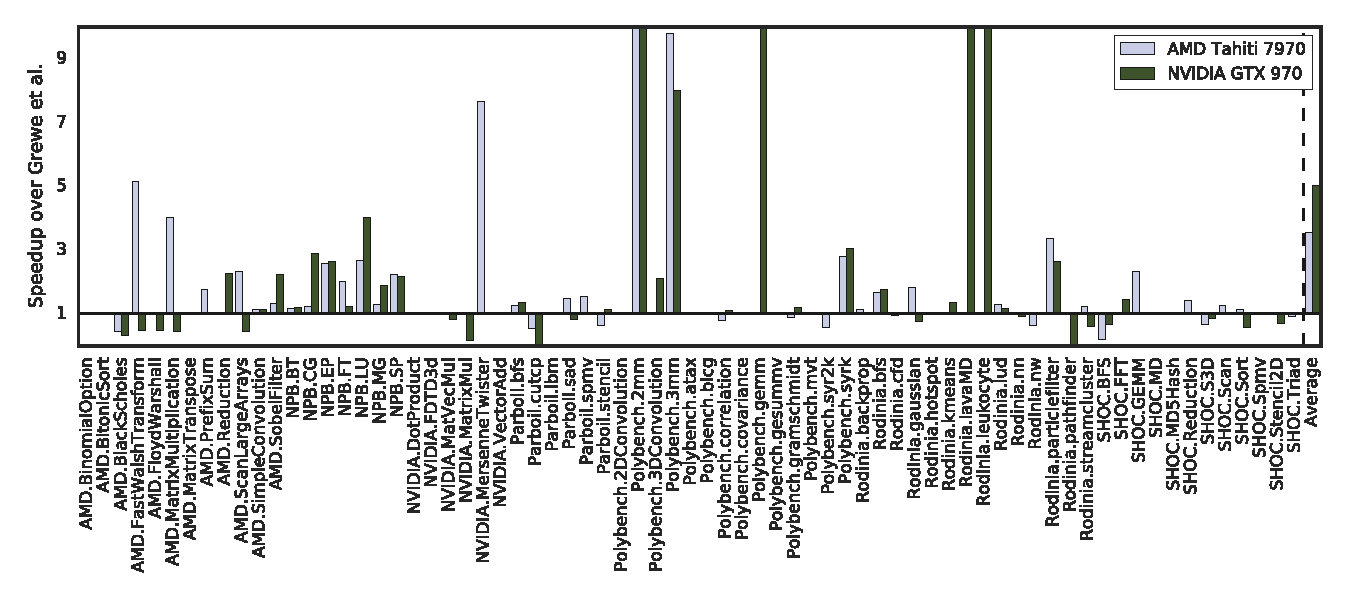
\includegraphics[width=1.45\textwidth,angle=270]{img/ex2}%
  \caption[Speedups of predictions using extended model over state-of-the-art]{%
    Speedups of predictions using an extended model over \citeauthor{Grewe2013} on both experimental platforms. Synthetic benchmarks and the additional program features outperform the original predictive model by a factor $3.56\times$ on AMD and $5.04\times$ on NVIDIA.%
  }%
  \label{fig:ex2}%
\end{figure}


\subsection{Comparison of Source Features}

As demonstrated in Section~\ref{sec:the-case-for-benchmark-generators}, the predictive quality of a model for a given point in the feature space is improved with the addition of observations from neighbouring points. By producing thousands of artificial programs modelled on the structure of real OpenCL programs, CLgen is able to consistently and automatically generate programs which are close in the feature space to the unseen benchmarks that are in the test set.

To quantify this effect, the static code features of Table~\ref{tab:clgen-cgo13-features-raw}, plus the branching feature discussed in the previous subsection, are used to measure the number of CLgen kernels generated with the same feature values as those of the benchmarks examined in the previous sections. Only static code features are examined to allow comparison with the GitHub kernels for which there is no automated method to execute and extract runtime features, and to enable comparison against code generated by CLSmith.

Figure~\ref{fig:clgen-nearest-neighbour} plots the number of exact feature vector matches as a function of the number of kernels. Out of 10,000 unique CLgen kernels, more than a third have static feature values matching those of the benchmarks, providing on average 14 CLgen kernels for each benchmark. This supports the underlying intuition: CLgen kernels, by emulating the way real humans write OpenCL programs, are concentrated in the same area of the feature space as real programs. Moreover, since the number of CLgen kernels that can be generated is unbounded, the exploration of the feature space can be continually refined. This is not the case for GitHub, where the number of kernels is finite. CLSmith rarely produces code similar to real-world OpenCL programs, with only 0.53\% of the generated kernels have matching feature values with benchmark kernels. The unique contribution of CLgen is its ability to generate many thousands of programs \textit{that are appropriate for predictive modelling}.

\begin{figure}
  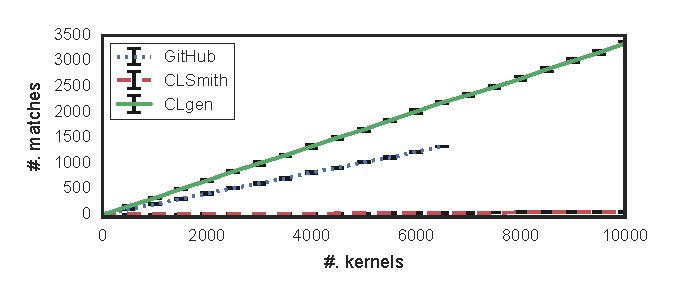
\includegraphics[width=\columnwidth]{img/closeness} %
  \caption[Number of kernels matching benchmark features]{%
    The number of kernels from GitHub, CLSmith, and CLgen with static code features matching the benchmarks. CLgen generates kernels that are closer in the feature space than CLSmith, and continues to do so long after the extent of the GitHub data set is exhausted. Error bars show the standard deviation from 10 random samplings.%
  }%
  \label{fig:clgen-nearest-neighbour}
\end{figure}


\section{Summary}
\label{sec:clgen-conclusion}

The quality of predictive models is bounded by the quantity and quality of programs used for training, yet there are typically only a few dozen common benchmarks available for experiments. This \emph{data scarcity challenge} (Section~\ref{subsec:challenge-scarcity}) limits the applicability of machine learning to compiler optimisations. This chapter presents a novel tool which is the first of its kind --- an entirely probabilistic program generator capable of producing an unbounded number of human-like programs. The approach applies deep learning over a huge corpus of publicly available code from GitHub to automatically infer the syntactical properties and practical usage of a programming language.

The tool generates synthetic programs which to trained eyes are indistinguishable from handwritten code. The approach is tested using a state-of-the-art predictive model, improving its performance by a factor of $1.27\times$. Synthetic benchmarks automatically exposed weaknesses in the feature set which, when corrected, further improved the performance by $4.30\times$.

Given the ability of generative models for performance characterisation, it is natural to hypothesise that a generator for unbounded programs may prove useful for compiler validation. Compared to benchmarking, compiler validation places very different requirements for how the synthesised code fragments are used. The following chapter presents techniques to adapt and extend the generative model to the challenging domain of compiler test case generation.
